%!TEX root = ../thesis.tex

本章では, 先行研究を基にした提案手法をデータの収集方法, 訓練時, テスト時の3節に分けて紹介する.

\section{手法1}

\subsection{データの収集方法}
\figref{Fig:old-method}にデータの収集方法を示す. 赤色の線である目標経路から平行に±0.10, ±0.20, ±0.30m離れた座標にロボットを配置する. そして, その座標ごとに目標経路に沿った向きを基準として±5度傾けて, 64×48のカメラ画像(RGB画像)とルールベース制御器によるナビゲーションの出力である角速度を\figref{Fig:collect-data2}のように収集する. これをGazeboのWillow Garageで\figref{Fig:willow-garage}に示すコースで一周行う.

% \vspace{10mm}

\begin{figure}[h]
  \centering
  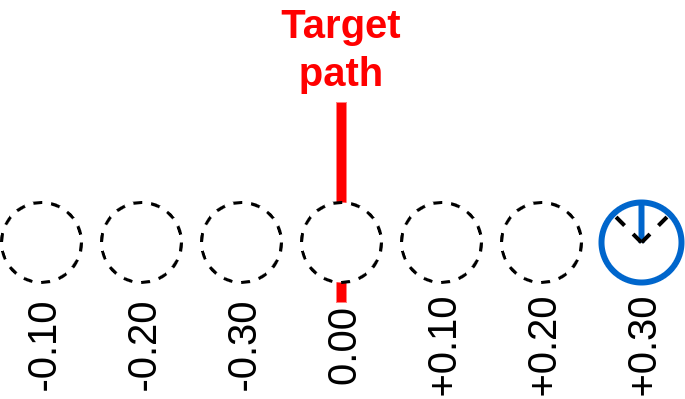
\includegraphics[keepaspectratio, scale=0.25]{images/old-method.png}
  \caption{Method of collecting data around the target route}
  \label{Fig:old-method}
  \end{figure}

\newpage
  \begin{figure}[h]
  \centering
  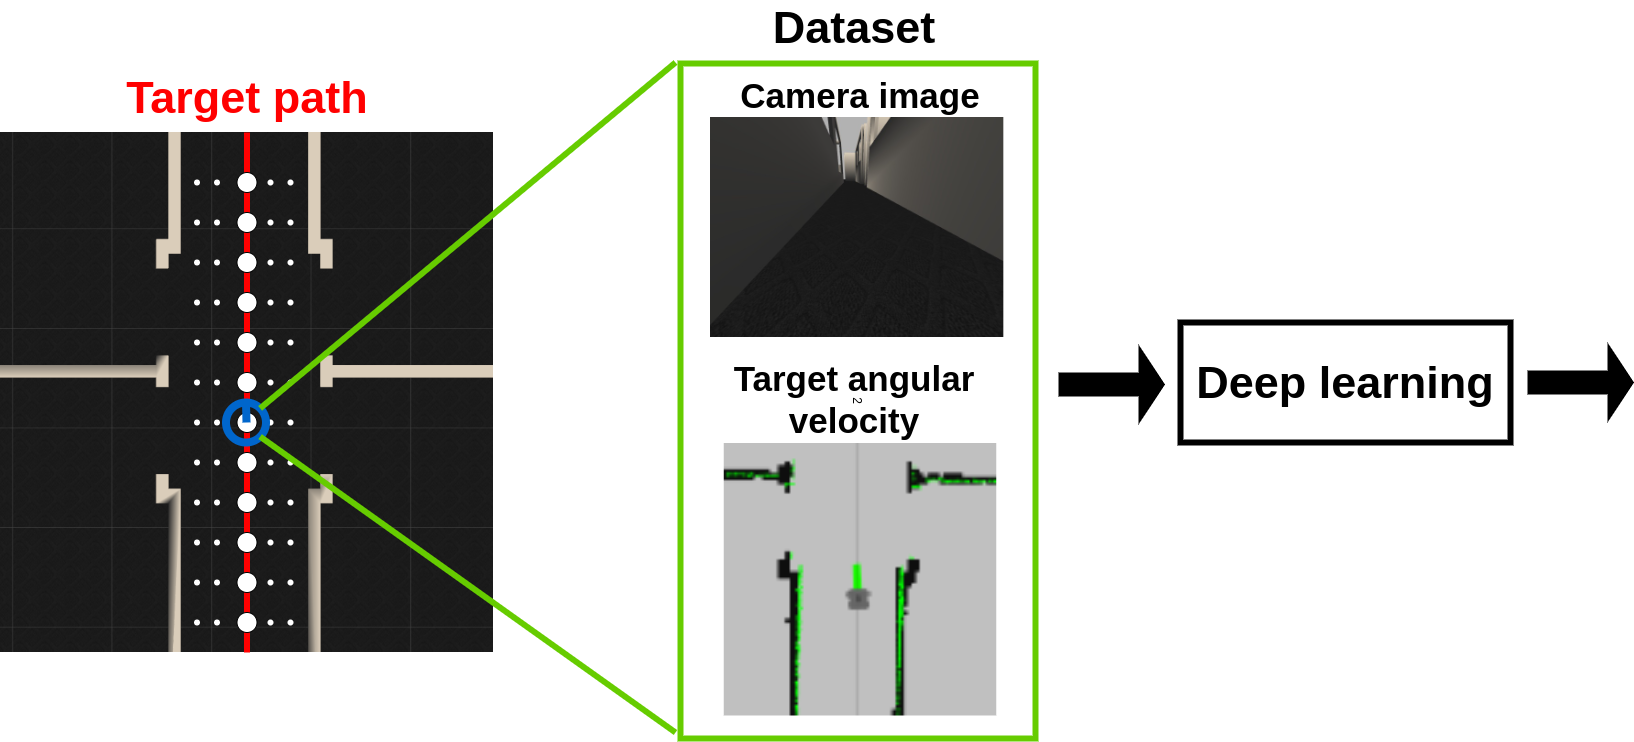
\includegraphics[keepaspectratio, scale=0.25]{images/collect-data2.png}
  \caption{Method of collecting data around the target route}
  \label{Fig:collect-data2}
  \end{figure}

\vspace{15mm}

\begin{figure}[h]
  \centering
  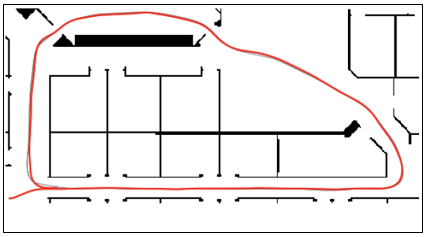
\includegraphics[keepaspectratio, scale=0.5]{images/willow-garage.png}
  \caption{Course to collect data}
  \label{Fig:willow-garage}
  \end{figure}

\newpage
\subsection{訓練時}
\subsubsection{ネットワークの構造}
\figref{Fig:cnn}に訓練時に用いたネットワークの構造を示す. 構造は, 入力層1, 畳み込み層3, 全結合層2, 出力層1の計7層から構成されている. 

\begin{figure}[h]
  \centering
  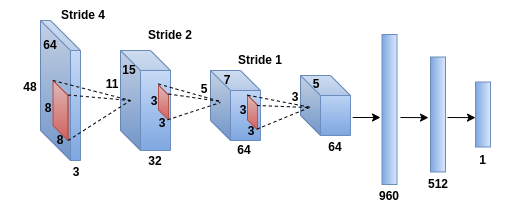
\includegraphics[keepaspectratio, scale=0.5]{images/cnn.png}
  \caption{Structure of network}
  \label{Fig:cnn}
  \end{figure}

\newpage
\section{手法2}

\subsection{データの収集方法}
\figref{Fig:collect-data}にデータの収集方法を示す. 赤色の線である目標経路から平行に±0.01, ±0.02, ±0.04, ±0.06, ±0.08, ±0.10, ±0.15, ±0.20, ±0.30m離れた座標にロボットを配置する. そして, その座標ごとに目標経路に沿った向きを基準として±5度傾けて画像とルールベース制御器によるナビゲーションの出力である角速度を\figref{Fig:collect-data2}のように収集する. これを\figref{Fig:willow-garage}に示すコースで一周行う. 

\vspace{10mm}

\begin{figure}[h]
  \centering
  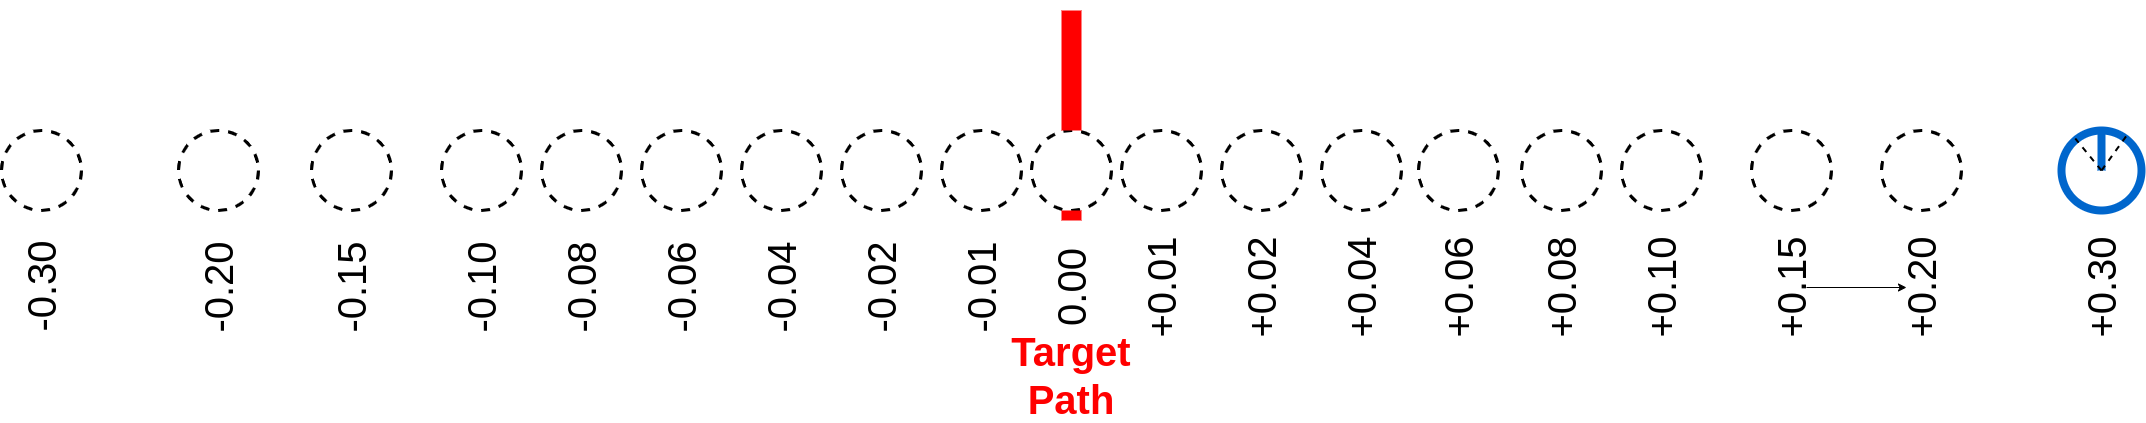
\includegraphics[keepaspectratio, scale=0.18]{images/collect-data.png}
  \caption{Method of collecting data around the target route}
  \label{Fig:collect-data}
  \end{figure}

\newpage
\section{訓練時}